% Chapter 4

\chapter{Stochastische Collocation}
Wie bereits die Monte-Carlo-Methode basieren auch stochastische Collocationsverfahren auf \emph{sampling}, d.h. der wiederholten Auswertung von vielen Zufallsexperimenten. Bei der Monte-Carlo-Methode werden die Punkte dabei abhängig von der gegebenen Verteilung unabhängig und zufällig gewählt. Die Konvergenz ist in einem stochastischen Sinne durch das Gesetz der großen Zahlen gegeben.\\
Dies ist ein großer Unterschied zu den hier vorgestellten stochastischen Collocationsverfahren. Für diese werden die Collocationspunkte nicht zufällig, sondern so gewählt, dass mithilfe von ihnen eine Polynominterpolation oder Quadratur möglich ist. Konvergenz ist dann abhängig davon, wie gut sich die approximierte stochastische Größe durch Polynome von Zufallsvariablen approximieren lässt.\\
Die beiden Ansätze \emph{Interpolation} und \emph{diskrete Projektion} (auch \emph{pseudospektraler Ansatz} genannt) werden für die stochastische KGG im Folgenden detailliert vorgestellt und miteinander verglichen.
\section*{Collocation für die stochastische KGG}
\todo[inline]{Algorithmen für Ansätze mit Pseudocode}
Die stochastische KGG (\ref{skgg}) für $d$ räumliche Dimensionen, $N$ stochastische Dimensionen und $y\in\R^N$ war definiert durch
\begin{align*}
\dtt{u}(t,x,y)&=\alpha(y) \Laplace_x u(t,x,y) - \beta(x,\omega)u(t,x,y), \: t>0, \, x\in \Torus^d\\
u(0,x,y)&=u_0(x,y), \: x\in \Torus^d\\
\dt{u}(0,x,y)&=v_0(x,y), \: x\in \Torus^d
\end{align*}
Im klassischen Sinne bedeutet Collocation, dass eine Approximation für eine diskrete Knotenmenge $\Theta_Y=\lbrace y_i\in\R^N\mid i=1,\dots,S\rbrace$ exakt ist. Auf die stochastische KGG übertragen, muss also für $y=y_i\in\Theta_Y$ die Lösung $u(t,x,y_i)$ für $x\in\Torus^d$ und $t>0$ vorliegen und die Approximation $w$ erfüllt $w(t,x,y_i)=u(t,x,y_i)$ für $i=1,\dots,S$. Da wir die exakte Lösung $u(t,x,y_i)$ nicht kennen, sondern für einen Zeitpunkt $T>0$ und eine Knotenmenge $\lbrace x_j\in\Torus^d\mid j=1,\dots,H\rbrace$ nur mithilfe des Strang-Splittings approximieren können, gilt für festes $x_j$ die Collocationsbedingung lediglich approximativ:
\[w(T,x_j,y_i)=u(T,x_j,y_i)\approx \tilde{u}(T,x_j,y_i),\quad i=1,\dots,S\]
Wir wählen daher $\tau$ so klein, dass dieser Fehler im Vergleich zum eigentlichen Collocationsfehler vernachlässigbar gering ist. Zur Vereinfachung der Notation nehmen wir im Folgenden an, die Lösung $u(T,x_j,y_i)$ liege exakt vor.

\section{Interpolation}
Sei $Y$ ein $N$-dimensionaler Zufallsvektor mit stochastisch unabhängigen Komponenten und $\Theta_Y\subset I_Y$ eine zu den Verteilungen von $Y_i$ passende $S$ elementige Knotenmenge. Seien weiter $\lbrace \Phi_m \mid |m|\le P \rbrace$ die zu den Verteilungen passenden gPC Basisfunktionen und im Folgenden mit $m=0,\dots,M=\binom{N+P}{P}-1$ durchnummeriert. Eine Diskussion zur Nummerierung findet man im vorherigen Kapitel.\\
Dann wählen wir als Interpolationspolynom die Funktion
\begin{equation}
\label{eqn:coll_interpol_basic}
w_M^{(j)}(Y)=\sum_{m=0}^M\hat{w}_m^{(j)}\Phi_m(Y)\in\Poly_P^N(Y),\quad j=1,\dots,H
\end{equation}
und fordern als Interpolationsbedingung
\[w_M^{(j)}(y_i)=u(T,x_j,y_i),\quad i=1,\dots,S, j=1,\dots,H\]
Die Notation macht klar, dass wir zu einem gegebenen Zeitpunkt $T>0$ und jedem festen Knotenpunkt $x_j$ die stochastische Funktion $u(T,x_j,Y)$ durch ein Polynom in $Y$ approximieren wollen.\\
Betrachten wir die Gleichung (\ref{eqn:coll_interpol_basic}) in den Knotenpunkten $y_i$ für jedes $i=1,\dots,S$, so können wir das entstehende System kompakt schreiben als
\begin{equation}
\label{eqn:interpol_compact}
A\hat{w}=u
\end{equation}
mit 
\begin{align*}
A&=(\Phi_m(y_i))_{i=1,\dots,S;m=0,\dots,M}\in\R^{S\times M+1}\\
\hat{w}&=(\hat{w}_m^{(j)})_{m=0,\dots,M;j=1,\dots,H}\in\R^{M+1\times H}\\
u&=(u(T,x_j,y_i))_{i=1,\dots,S;j=1,\dots,H}\in\R^{S\times H}\\
\end{align*}
Für jeden Knotenpunkt $x_j$ ist ein lineares Gleichungssystem der Größe $S\times M+1$ zu lösen. Die obige Schreibweise erlaubt es in vielen Programmiersprachen die Systeme gleichzeitig zu lösen und bietet somit einen starken Laufzeitvorteil gegenüber dem Lösen von $H$ separaten Gleichungen. Um sicherzustellen, dass das System nicht unterbestimmt ist, muss gelten $S\ge M+1=\binom{N+P}{P}$. Ist $S\neq M+1$, so verwenden wir die Pseudoinverse von $A$. Später werden wir an verschiedenen Beispielen Konsequenzen dieser Bedingung genauer betrachten.
\begin{mathbem}
In Gleichung (\ref{eqn:gpc_approx_exp}) wurde gezeigt, dass sich der Erwartungswert an der Stelle $x_j$ approximieren lässt durch
\[\E[u(t,x_j,Y)]\approx \hat{w}_0^{(j)}\]
Da die Gleichungen gekoppelt sind, müssen aber trotzdem auch alle anderen $\hat{w}_m$ berechnet werden.
\end{mathbem}
\subsection{Wahl der Interpolationspunkte}
\label{chapter:interpolation_points}
Wir wollen direkt am Anfang darauf hinweisen, dass im Mehrdimensionalen für $N>1$ die Wahl der Knotenpunkte für die Interpolation ein nicht vollständig verstandenes Problem darstellt. Das Konzept der Lagrange-Interpolation, die im Eindimensionalen für jede beliebige Knotenmenge möglich ist, lässt sich wie in \autocite{San07} gezeigt konzeptuell auf den mehrdimensionalen Fall erweitern. Allerdings benötigt sie die entsprechende Bedingung $\det(A)\neq 0$, welche besagt, dass die Interpolation durch die gegebenen Knotenpunkte eindeutig ist. Die Beziehung dieser Bedingung zur Wahl der Knotenpunkte stellt ein "'komplexes Problem"' dar.
\subsubsection*{Grundlagen der eindimensionalen Interpolation}
Der Satz von Cauchy ist der erste Orientierungspunkt für die Abhängigkeit der Interpolationsgüte zur Wahl der Knotenpunkte für den eindimensionalen Fall und einem kompakten Intervall.
\begin{maththeorem}[Cauchy]
Sei $f\in C^{S}[-1,1]$ eine $S$ mal stetig differenzierbare Funktion. Dann ist für jede Knotenmenge $\lbrace y_1,\dots,y_{S}\rbrace$ und $y\in[-1,1]$ der Interpolationsfehler gegeben durch
\[f(y)-\mathcal{Q}_{S}f=\frac{f^{(S)}(\xi)}{S!}\prod_{i=1}^{S}(y-y_i),\quad \xi\in [-1,1]\]
\end{maththeorem}

Da die Funktion gegeben ist, hat man keinen Einfluss auf die Ableitung $f^{(S)}$. Wegen
\[\norm{f(y)-\mathcal{Q}_{S}f}\le \frac{\norm{f^{(S)}}_\infty}{S!}\underbrace{\norm{\prod_{i=1}^{S}(y-y_i)}}_{=\norm{w(y)}}\]
ist es somit das Ziel, den Term $\norm{w(y)}$ abhängig von der Norm zu minimieren.
\begin{mathbem}[\chebyspace Interpolation]
\label{bem:cheby}
Die Nullstellen $y_i=\cos\left(\pi\frac{2i-1}{2S+2}\right)$, für $i=1,\dots,S+1$, der \chebyspace Polynome $T_{S+1}(y)=\cos((S+1)\arccos(y))$ minimieren den Ausdruck $\norm{w(y)}_\infty$ auf $[-1,1]$ und bieten auf $[-1,1]$ optimale Interpolationsgüte. Es gilt 
\[\norm{f(y)-\mathcal{Q}_{S+1}f}_\infty\le \frac{\norm{f^{(S+1)}}_\infty}{2^S(S+1)!}\]
\end{mathbem}
Die \chebyspace Polynome bilden eine Orthogonalbasis bezüglich $\langle \cdot,\cdot\rangle_{L_w^2[-1,1]}$ mit $w(y)=(1-y^2)^{-\onehalf}$. Eine Idee ist es nun, auch Nullstellen anderer orthogonalen Polynombasen als Knotenpunkte zu verwenden um ähnliche Approximationsergebnisse auf nicht-kompakten Intervallen zu erhalten.
\begin{maththeorem}
\label{th:interpol_and_proj}
Sei $\lbrace \Phi_m\in\Poly_m\mid m=0,\dots,M\rbrace\subset L_w^2(I)$ eine Orthonormalbasis von Polynomen und $(y_i,a_i)_{i=0,\dots,M}$ eine Quadraturformel mit Exaktheitsgrad $2M$ bezüglich $w$ und $y_i\neq y_j,i\neq j$, d.h. \[\int_I p(y)w(y)dy=\sum_{i=0}^M a_ip(y_i),\quad p\in\Poly_{2M}\]
Sei weiter das Interpolationspolynom  $\mathcal{Q}_Mf$ einer Funktion $f\colon I\to\R$ bezüglich den Interpolationspunkten $\lbrace y_i\mid i=0,\dots,M\rbrace$ beschrieben durch
\[\mathcal{Q}_Mf(y)=\sum_{m=0}^M\hat{w}_m\Phi_m(y)\]
Die Koeffizienten $\hat{w}_m$ werden in Analogie zu (\ref{eqn:interpol_compact}) berechnet durch das Lösen des linearen Gleichungssystems
\[A\hat{w}=\hat{f}\]
Dann ist \[\hat{w}_i=\sum_{j=0}^M\Phi_i(y_j)a_jf(y_j)\approx \int_I \Phi_i(y)f(y)w(y)dy,\quad i=0,\dots,M\]
\end{maththeorem}
\begin{proof}
Es ist $A_{ij}=\Phi_j(y_i)$. Da wir uns im eindimensionalen Fall befinden ($N$=1) ist die Vandermonde-artige Matrix $A$ invertierbar, da die $\Phi_i$ eine Basis bilden und die $y_i$ paarweise verschieden sind. Es gilt für $\widetilde{w}_i\coloneqq \sum_{j=0}^M\Phi_i(y_j)a_jf(y_j)$ und $\widetilde{w}\coloneqq (\widetilde{w}_i)^T$
\begin{align*}
\left(A\widetilde{w}\right)_i&=\sum_{j=0}^M\Phi_j(y_i)\widetilde{w}_j\\
&=\sum_{j=0}^M\Phi_j(y_i)\sum_{k=0}^M\Phi_j(y_k)a_kf(y_k),\quad \text{Interpol.:} f(y_k)=\sum_{\ell=0}^M\hat{w}_\ell\Phi_\ell(y_k)\\
&=\sum_{\ell=0}^M\hat{w}_\ell \sum_{j=0}^M\Phi_j(y_i)\sum_{k=0}^M\Phi_j(y_k)a_k\Phi_\ell(y_k)\\
&\stackrel{\text{deg}(\Phi_j\Phi_\ell)\le 2M}{=}\sum_{\ell=0}^M\hat{w}_\ell\sum_{j=0}^M\Phi_j(y_i)\underbrace{\int_I\Phi_j(y)\Phi_\ell(y)w(y)dy}_{=\delta_{j\ell}}\\
&=\sum_{\ell=0}^M\hat{w}_\ell\Phi_\ell(y_i)=f(y_i)=\hat{f}_i
\end{align*}
Also gilt $A\widetilde{w}=\hat{f}=A\hat{w}$ und da $A$ regulär ist somit $\widetilde{w}=\hat{w}$.
\end{proof}
\begin{mathbem}
Wir wollen nun dem technischen Satz \ref{th:interpol_and_proj} Leben einhauchen und seine Relevanz verdeutlichen.
\begin{itemize}
\item
Die vorausgesetzte Existenz einer Quadraturformel aus $M+1$ verschiedenen Quadraturpunkten und Exaktheitsgrad $2M$ ist durch die später vorgestellte Gauss-Quadratur erfüllt. Die Quadraturpunkte sind dabei die Nullstellen des $M+1$-ten Basispolynoms und daher paarweise verschieden. Die Quadraturgewichte lassen sich über die erste Komponente des zugehörigen normierten Eigenvektors bestimmen.
\item
Wir sehen, dass sich im Eindimensionalen bei bekannter Quadraturformel die Interpolationskoeffizienten $\hat{w}_m$ auch einzeln ohne Lösen eines linearen Gleichungssystems berechnen lassen. Diese Darstellung führt auf den später vorgestellten zweiten Ansatz zur stochastischen Collocation.
\item
Die Darstellung $\hat{w}_i=\sum_{j=0}^M\Phi_i(y_j)a_jf(y_j)$ kann als Approximation an die Koeffizienten $\int_I \Phi_i(y)f(y)w(y)dy$ der Bestapproximation $P_Mf$ in $L_w^2(I)$ aufgefasst werden. Mithilfe der Dreiecksungleichung lässt sich dann der Fehler der Interpolation beschreiben durch
\begin{align*}
&\norm{\mathcal{Q}_Mf-f}_{L_w^2}\le \underbrace{\norm{P_Mf-f}_{L_w^2}}_{\text{Fehler der Bestapproximation}}+\underbrace{\norm{\mathcal{Q}_Mf-P_Mf}_{L_w^2}}_{\text{Aliasing Fehler}}\\
&=\norm{\mathcal{Q}_Mf-P_Mf}_{L_w^2}+\norm{\sum_{m=0}^M\left(\sum_{j=0}^M\Phi_m(y_j)a_jf(y_j)\right)\Phi_m-\sum_{m=0}^M\left(\int_I\Phi_m(y)f(y)w(y)dy\right)\Phi_m}_{L_w^2}\\
&\stackrel{\text{Parseval}}{=}\norm{\mathcal{Q}_Mf-P_Mf}_{L_w^2}+\sqrt{\sum_{m=0}^M\left(\sum_{j=0}^M\Phi_m(y_j)a_jf(y_j)-\int_I\Phi_m(y)f(y)w(y)dy\right)^2}
\end{align*}
Schlussendlich lässt sich also der Fehler der Interpolation durch den Fehler der Bestapproximation in $L_w^2$ und einen Quadraturfehler bezüglich der Gewichtsfunktion $w$ beschreiben. Für den Fehler der Bestapproximation erwarten wir nach Xiu spektrale Konvergenz. Finden wir eine zur Gewichtsfunktion $w$ passende Quadraturformel, so hat lediglich die Glattheit von $f$ Einfluss auf den Quadraturfehler, da $\Phi_m$ als Polynom bei hinreichend hoher Ordnung exakt integriert wird.
\end{itemize}
\end{mathbem}
\begin{mathbsp}
Wir vergleichen anhand von \nameref{trial:1} für $d=1$ zwei Möglichkeiten zur Wahl der Interpolationspunkte. Da $Y$ eine Gleichverteilung zugrunde liegt, verwenden wir die normalisierten Legendre-Polynome $L_0,\dots,L_M$. Als Interpolationspunkte $y_i$ wählen wir dann
\begin{enumerate}
\item die $M+1$ Nullstellen des Legendre-Polynoms vom Grad $M+1$ (genannt \textit{full\_tensor}).
\item die $M+1$ Nullstellen des \chebyspace Polynoms vom Grad $M+1$ (siehe Bemerkung \ref{bem:cheby}).
\end{enumerate}
In Abbildung \ref{fig:collocation_trial1} ist die Approximationsgüte der Interpolation dargestellt, links für $\tau=0.001$ und rechts für $\tau=0.0001$, gemessen durch die Fehler an den Erwartungswert und die Varianz. Man erkennt, dass die \chebyspace Interpolation langsamer konvergiert als die Legendre-Interpolation. Die Konvergenz stoppt bei einer gewissen Genauigkeit, die abhängig ist von $\tau$. Dies ist dadurch begründet, dass die Punkte $u(T,x_j,y_i)$ nicht exakt vorliegen sondern lediglich mithilfe eines Strang-Splittings mit Schrittweite $\tau$ approximiert werden. Dies betont die Wichtigkeit der Wahl eines kleinen $\tau$, allerdings bedeutet ein kleineres $\tau$ gleichzeitig eine entsprechende multiplikative Vergrößerung der Berechnungszeit.
\begin{figure}[!htb]
\minipage{0.5\textwidth}
  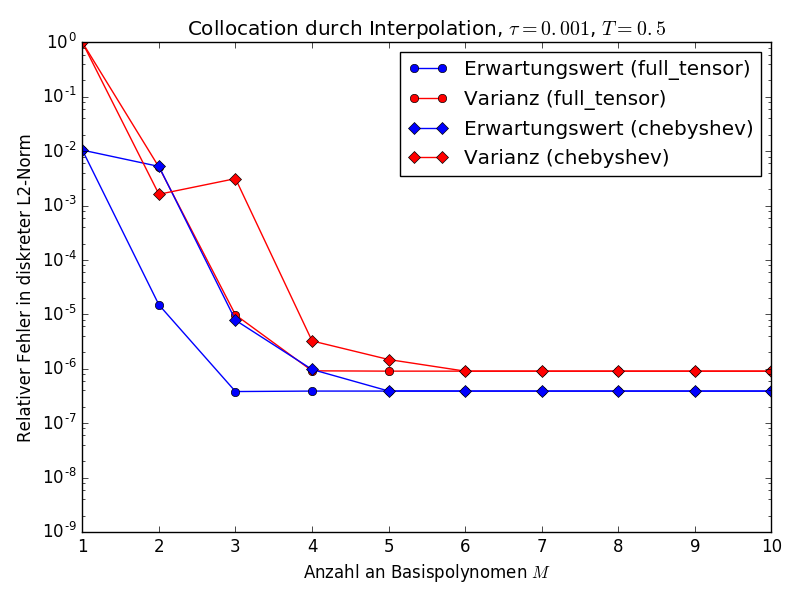
\includegraphics[width=\linewidth]{Figures/collocation_mi_trial1_tau001.png}
\endminipage
\minipage{0.5\textwidth}
  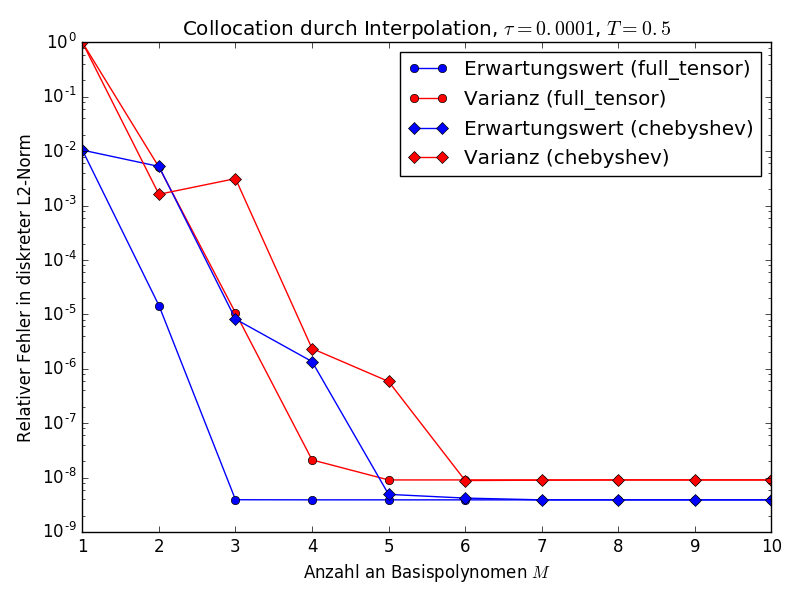
\includegraphics[width=\linewidth]{Figures/collocation_mi_trial1_tau0001.png}
\endminipage
\caption{Vergleich von verschiedenen Interpolationspunkten und der Abhängigkeit der bestmöglichen Interpolation von der Genauigkeit der Interpolationspunkte anhand von \nameref{trial:1} zum Zeitpunkt $T=0.5$ und für $d=1$.}
\label{fig:collocation_trial1}
\end{figure}
\end{mathbsp}
\subsubsection*{Mehrdimensionale Interpolation durch volles Tensorprodukt}
Eine mögliche Wahl für $N>1$ die Menge der Interpolationspunkte $\Theta_Y^N$ zu einem gegebenem Zufallsvektor $Y$ der Dimension $N$ zu wählen, ist gegeben durch das volle Tensorprodukt
\[\Theta_Y^N=\Theta_{Y_1}\otimes \dots \otimes \Theta_{Y_N},\quad \Theta_{Y_i}\subset I_{Y_i}\]
Dann gilt für die Anzahl der Interpolationspunkte $S=S_1 \dots S_N$. Ist die Anzahl an Basispolynomen $M+1$ fest, so ist es schwierig die Bedingung $S=M+1$ exakt zu erfüllen. Wir fordern daher, dass $S_1=\dots=S_N$ und $S\ge M+1$ minimal. Dieser Ansatz wird in Abbildungen durch \textit{full\_tensor} gekennzeichnet.
\subsubsection*{Mehrdimensionale Interpolation durch pseudo-dünne Gitter}
Eine weitere Idee für die mehrdimensionale Interpolation, welche die Gleichung $M+1=\binom{N+P}{P}$ exakt erfüllt, ist mit $S_1=\dots=S_N$ die Wahl
\[\Theta_Y^N=\lbrace (y_{m_1},\dots,y_{m_N})\in \Theta_{Y_1}\otimes \dots \otimes \Theta_{Y_N} \mid |m|\le P,m\in\N_0^N \rbrace \]
Es wird somit jedem Multi-Index $m\in\N_0^N$ genau ein mehrdimensionaler Interpolationspunkt $y$ zugewiesen und es gilt $M+1=S$. Die Matrix im Interpolationsansatz ist dadurch quadratisch und besitzt für kleine $P$ eine geringere Kondition.\\[0.1cm]
Die Wahl der Nummerierung der eindimensionalen Interpolationspunkte ist entscheidend. Für Legendre- oder Hermite-Polynome bietet sich eine betragsmäßig aufsteigende Sortierung der Punkte an, da diese symmetrisch um $0$ verteilt sind. Für Jacobi- und Laguerre-Polynome beobachten wir in Abbildung \ref{fig:poly_roots} keine Symmetrie. Dennoch gilt die Eigenschaft von Orthogonalpolynomen, dass die Nullstellen eines Polynoms höheren Grades zwischen den Nullstellen des vorherigen Polynoms zu finden sind. Wir sortieren die Nullstellen auf- oder absteigend, um eine möglichst repräsentative Auswahl der Punkte des vollen Tensorprodukts zu bekommen. Die Idee ist dadurch motiviert, dass so die Struktur der Entwicklung der Nullstellen einer Polynombasis berücksichtigt wird, auch wenn diese keine eindeutige Schachtelung aufweisen.\\
Dieser Ansatz wird in Abbildungen durch \textit{pseudo\_sparse} gekennzeichnet. Er ist eine Heuristik, um den Einfluss der Überbestimmtheit des zu lösenden Systems besser zu verstehen und sollte nicht als robuste Methode für mehrdimensionale Interpolation aufgefasst werden.\\
\begin{figure}[!htb]
\minipage{0.5\textwidth}
  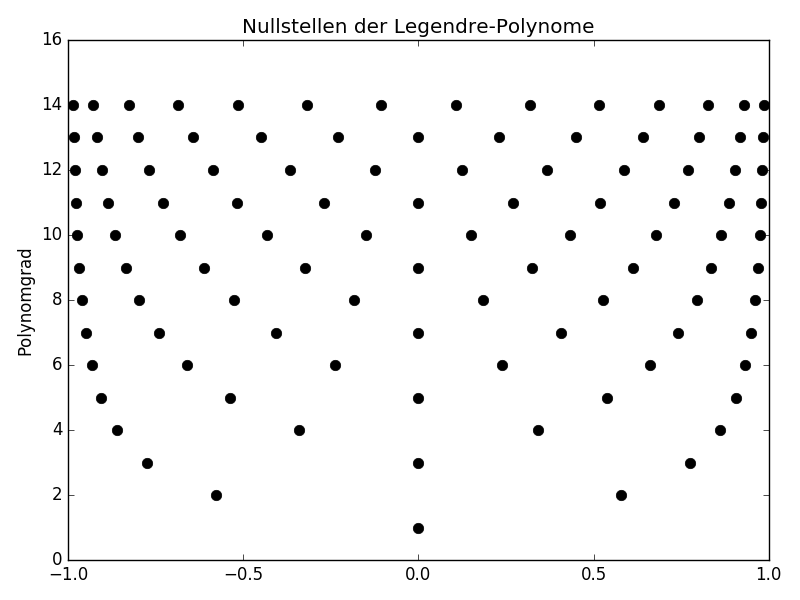
\includegraphics[width=\linewidth]{Figures/roots_legendre.png}
  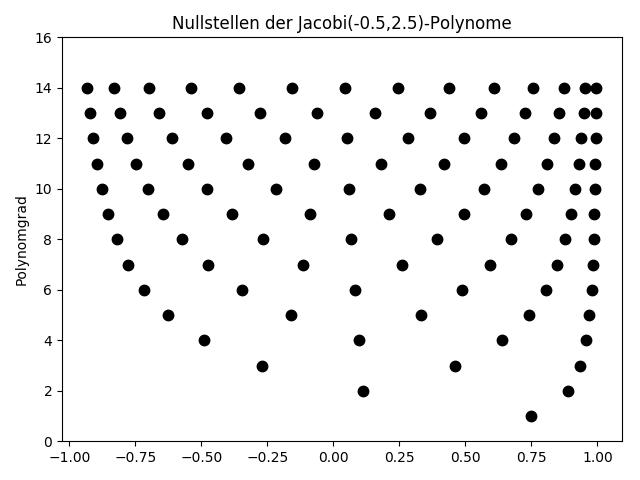
\includegraphics[width=\linewidth]{Figures/roots_jacobi.png}
\endminipage
\minipage{0.5\textwidth}
  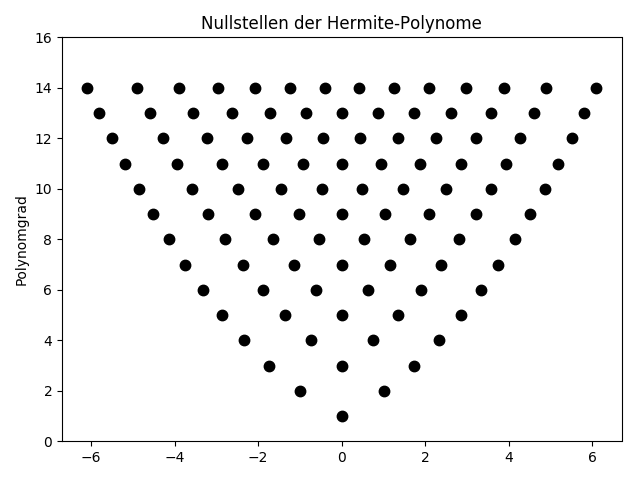
\includegraphics[width=\linewidth]{Figures/roots_hermite.png}
  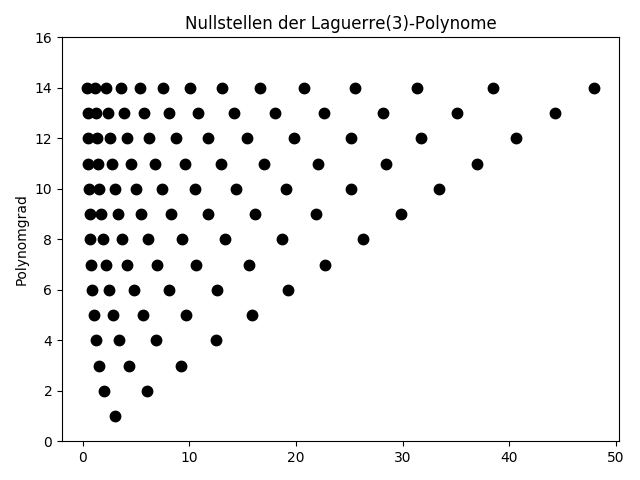
\includegraphics[width=\linewidth]{Figures/roots_laguerre.png}  
\endminipage
\caption{Nullstellen verschiedener Orthogonalbasen von Polynomen mit steigendem Grad.}
\label{fig:poly_roots}
\end{figure}
Ein Beispiel sei für $N=2$ und $P=14$ gemacht, wo für Legendre- und Laguerre-Polynome die Interpolationspunkte des pseudo-dünnen Gitters und des vollen Tensorprodukts in Abbildung \ref{fig:roots_two_dim} dargestellt sind.\\
\begin{figure}[!htb]
\centering
\minipage{0.5\textwidth}
  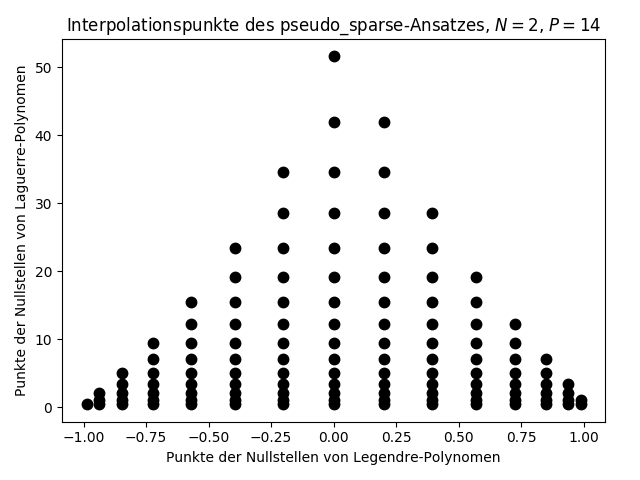
\includegraphics[width=\linewidth]{Figures/roots_pseudo_sparse.png}
\endminipage
\minipage{0.5\textwidth}
  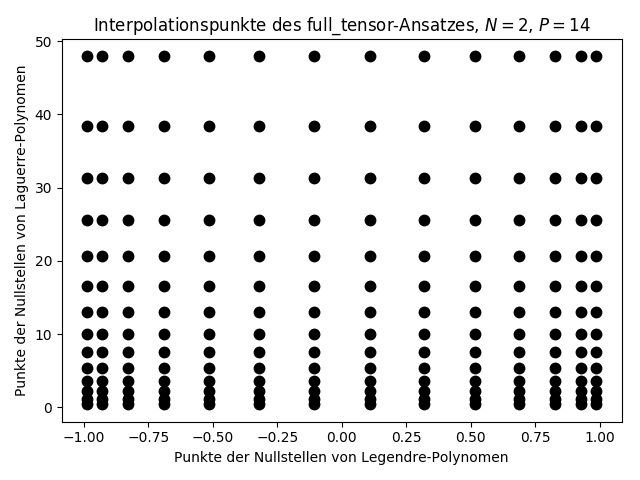
\includegraphics[width=\linewidth]{Figures/roots_full_tensor.png}
\endminipage
\caption{Interpolationspunkte für den pseudo-dünne Gitter Ansatz und das volle Tensorprodukt für die Nullstellen der Legendre- und Laguerre(3)-Polynome mit $N=2$ und $P=14$.}
\label{fig:roots_two_dim}
\end{figure}

Wir werden später basierend auf Smolyaks Konstruktion einen effizienteren dünne Gitter Ansatz kennen lernen, der nicht nur für Interpolation verwendbar ist, sondern sich auch auf generelle Operatoren übertragen lässt. Dieser basiert allerdings auf vollen Tensorprodukten von Operatoren und ist daher nur übertragbar, wenn wir volle Tensorprodukte von Polynombasen zulassen (d.h. ohne die zusätzliche Bedingung $|m|\le P$). Da dies einen erheblichen Rechenaufwand impliziert, werden wir keine dünnen Gitter Ansätze für die Interpolation verwenden.
\subsection{Algorithmus}
In Algorithmus \ref{alg:collocation_mi} ist das Collocationsverfahren für den eindimensionalen Fall $d=1$ skizziert. Diese Variante der Collocation durch Interpolation wird in der Literatur auch mit \emph{Matrix-Invertierung} (MI) bezeichnet. Die Matrix $A$ muss nicht explizit invertiert werden, trotzdem besteht der Kern des Verfahrens aus dem Lösen der linearen Gleichungssysteme.\\
\begin{tabular}{c|c}
Parameter & \\
\hline
$H$ & Anzahl an Punkten der Ortsdiskretisierung\\
$\kappa\in [0,1]$ & Gewicht für das Splittingverfahren zur Approximation von $u(T,x,Y)$\\
$Y$ & $N$-dimensionaler Zufallsvektor zu dem eine gPC-Basis existiert\\
$M+1$ & Anzahl an multivariaten gPC-Basispolynomen\\
$S$ & Anzahl an Interpolationspunkten gemäß einer der möglichen Ansätze
\end{tabular}
\begin{algorithm}[ht]
    \caption{Collocation durch Interpolation mithilfe von Matrix-Invertierung.}
    \label{alg:collocation_mi}
    \begin{algorithmic}[1] % The number tells where the line numbering should start
        \Function{Collocation\_Interpolation\_MI}{$H, u_0, v_0, \alpha,\beta,\kappa,Y, M, S,\tau, T$} 
            \State $\Phi_m\gets$ $m$-te orthonormale gPC-Basis-Funktion zu $Y$, $\quad m=0,\dots,M$
            \State $y_i\gets$ (multivariate) Interpolationspunkte (siehe Kapitel \ref{chapter:interpolation_points}), $\quad i=1,\dots,S$
            \State $A\gets (\Phi_m(y_i))_{i=1,\dots,S;m=0,\dots,M}\in\R^{S\times M+1}$
            \For{$i=1,\dots,S$}
           		\State $\tilde{u}_{ij}\gets \text{Fast\_Strang}(H,u_0(\cdot, y_i),v_0(\cdot, y_i),\alpha(y_i),\beta(\cdot, y_i),\kappa,\tau,T)_j$
           	\EndFor
            \State $u\gets (\tilde{u}_{ij})_{i=1,\dots,S;j=1,\dots,H}\in\R^{S\times H}$
            \State $\hat{w}\gets A^{-1}u\in\R^{S\times H}$
            \State \Comment{Lösen der linearen Gleichungssysteme, evtl. mit Pseudoinversen}
			\State $\mu\gets \hat{w}_{0,j=1,\dots,H}$ \Comment{Approximation an Erwartungswert}
			\State $\sigma^2_j\gets \sum_{m=1,\dots,M}\hat{w}^2_{mj}$\Comment{Approximation an Varianz an der Stelle $x_j$}
			\State \textbf{return} $\mu,\sigma^2$ \Comment{Approximation an Erwartungswert und Varianz}        
        \EndFunction
    \end{algorithmic}
\end{algorithm}
\subsection{Vergleiche der Ansätze}
Wir reduzieren uns für $N=1$ auf die Nullstellen derjenigen Orthogonalpolynome, die gemäß des gPC zu der Verteilung von $Y$ gehören. Für das kompakte Interval $I=[-1,1]$ wäre es ebenso möglich die \chebyspace Interpolationspunkte zu verwenden. Diese bieten aber nach unseren Beobachtungen keinen Vorteil.\\
Für $N>1$ besteht die Möglichkeit das volle Tensorprodukt der jeweiligen eindimensionalen Interpolationspunkte zu den Komponenten von $Y$ zu wählen. Da dies jedoch im Allgemeinen mehr Punkte umfasst als die vorhandenen $M+1$ Polynome, ist das lineare Gleichungssystem überbestimmt und wir beobachten eine hohe Kondition der Matrix. Dies sorgt insbesondere dafür, dass die Approximation der Varianz, welche jede Komponente des Lösungsvektors benötigt, bereits für $P>3$ instabil ist.\\
Anhand der \nameref{trial:8} aus dem Appendix mit $N=4$ vergleichen wir die beiden Ansätze in Abbildung \ref{fig:collocation_trial8}. 
\begin{figure}[!htb]
\centering
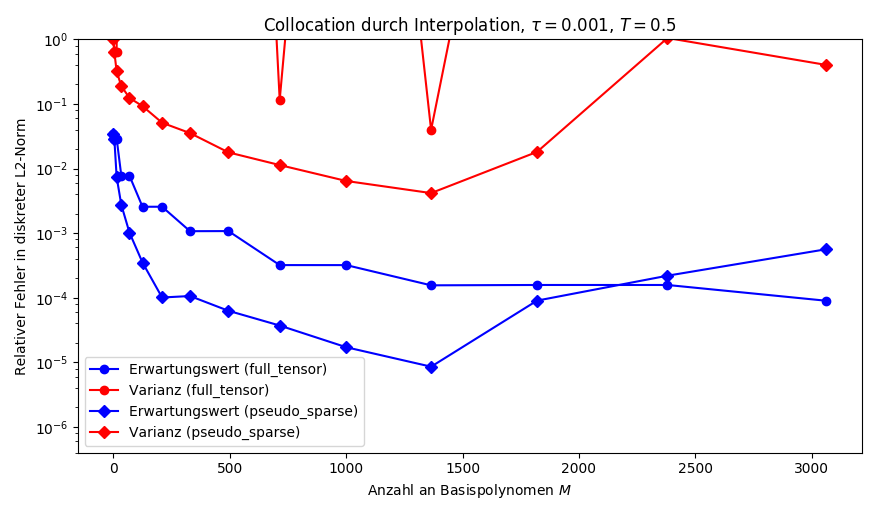
\includegraphics[width=\linewidth]{Figures/collocation_mi_trial8_ft_pseudosparse.png}
\caption{Approximation des Erwartungswerts und der Varianz von \nameref{trial:8} mithilfe von Collocation durch Interpolation und verschiedenen Ansätzen bis zu $P=14$.}
\label{fig:collocation_trial8}
\end{figure}
Wir sehen, dass sich der Erwartungswert mit beiden Ansätzen approximieren lässt. Bis zu $P=11$ ist die Approximation mit dem pseudo\_sparse Ansatz dabei um einen Faktor 10 genauer. Die Kondition der Matrix ist für $P=11$ jedoch bereits in der Größenordnung $\mathcal{O}(10^{13})$ mit wachsender Tendenz, was Approximationen mit $P>11$ zunehmend schlechter werden lässt.\\
Die Varianz ist durch das überbestimmte System beim full\_tensor Ansatz nicht berechenbar (für $P=9$ ergibt sich ein System der Größe $6^4\times \binom{4+9}{9} =1296\times 715$). Erhöht man $P$ weiter, so beobachtet man auch für den pseudo\_sparse Ansatz zunehmende Instabilität.

\section{Diskrete Projektion}
Der zweite Ansatz zur stochastischen Collocation basiert auf der Bestapproximation in $L_{\rho_Y}^2$.
\begin{mathdef}[Diskrete Projektion]
Sei $Y$ ein Zufallsvektor und $\Phi_m(Y)$ für $m=0,\dots,M$ die zugehörigen orthonormalen gPC Basisfunktionen. Dann ist die Bestapproximation der sKGG zu einem Zeitpunkt $T>0$ und für eine Stelle $x_j$ definiert als
\[P_Mu(T,x_j,Y)=\sum_{m=0}^M\hat{u}_m^{(j)}\Phi_m(Y)\]
mit Koeffizienten
\[\hat{u}_m^{(j)}=\E[u(T,x_j,Y)\Phi_m(Y)]=\int_{I_Y} u(T,x_j,y)\Phi_m(y)\rho_Y(y)dy\]
Ist nun $(y_i,a_i)_{i=0,\dots,Q}$ eine Quadraturformel für das Gewicht $\rho_Y$, so ist die diskrete Projektion definiert als
\[w_{M,Q}(T,x_j,Y)=\sum_{m=0}^M\hat{w}_m^{(j)}\Phi_m(Y)\] wobei für die Koeffizienten gilt
\[\hat{w}_m^{(j)}=\sum_{i=0}^Qu(T,x_j,y_i)\Phi_m(y_i)a_i\approx \int_{I_Y} u(T,x_j,y)\Phi_m(y)\rho_Y(y)dy\]
\end{mathdef}
Satz \ref{th:interpol_and_proj} zeigt, dass für $Q=M$ und eine Quadraturformel mit paarweise verschiedenen Quadraturpunkten und Exaktheitsgrad $2M$ die beiden Ansätze im Eindimensionalen äquivalent sind. Aus der Bemerkung nach Satz \ref{th:interpol_and_proj} folgt auch, dass sich der Fehler der diskreten Projektion mithilfe der Dreiecksungleichung durch den Fehler der Bestapproximation und einen Quadraturfehler, den Aliasing Fehler, abschätzen lässt.

\subsection{Gauss-Quadratur im Eindimensionalen}
Wir wollen nun eine möglichst exakte Quadraturformel konstruieren, welche auf natürliche Weise das jeweilige Gewicht $\rho$ des Integrals berücksichtigt.
\begin{maththeorem}[Gauss-Quadratur]
Sei $Q_0,\dots,Q_{n+1}\in L_\rho^2(I)$ eine Orthogonalbasis von Polynomen bezüglich des Gewichts $\rho$. Es sei $\text{deg}(Q_j)=j$ für $j=0,\dots,n+1$. Seien $y_0,\dots,y_n$ die Nullstellen des Polynoms $Q_{n+1}$. Dann ist die Quadraturformel $(y_i,a_i)$ mit 
\[\int_If(y)\rho(y)dy\approx \sum_{i=0}^na_if(y_i)\]
und 
\[a_i=\int_I \rho(y)\underbrace{\prod_{j\neq i} \frac{y-y_j}{y_i-y_j}}_{=\ell_i(y)}dy\]
exakt für alle Polynome vom Grad höchstens $2n+1$.
\end{maththeorem} 
\begin{proof}[Beweisskizze]
Sei $f$ ein Polynom vom Grad höchstens $2n+1$ und 
\[f(y)=Q_{n+1}(y)\underbrace{p(y)}_{deg \le n}+\underbrace{r(y)}_{deg \le n}\]
eine durch Polynomdivision erhaltene Zerlegung von $f$. Da die $y_i$ Nullstellen von $Q_{n+1}$ sind, gilt
\[f(y_i)=r(y_i),\quad i=0,\dots n\]
Dann ist
\[\int_If(y)\rho(y)dy=\underbrace{\int_IQ_{n+1}(y)p(y)\rho(y)dy}_{=0}+\int_Ir(y)\rho(y)dy\]
da $Q_{n+1}$ orthogonal zum Raum aller Polynome vom Grad höchstens $n$ ist.\\
Die interpolatorischen Quadraturformeln (wie beispielsweise die Newton-Cotes-Formeln) mit den Gewichten $a_i$, die über das gewichtete Integral der Lagrange-Polynome $\ell_i$ definiert werden, sind exakt für Polynome vom Grad höchstens $n$. Somit gilt
\[\int_If(y)\rho(y)dy=\int_Ir(y)\rho(y)dy=\sum_{i=0}^{n}a_ir(y_i)=\sum_{i=0}^{n}a_if(y_i)\]
\end{proof}
\begin{mathbem}
Wir nennen an dieser Stelle noch einige praktische Hinweise zur Gauss-Quadratur.
\begin{itemize}
\item Die Gauss-Quadraturformel zur entsprechenden gPC Basis erfüllt die Voraussetzungen an die Quadraturformel von Satz \ref{th:interpol_and_proj}.
\item Die Nullstellen $y_i$ lassen sich als die Eigenwerte einer symmetrischen Tridiagonalmatrix mithilfe des Golub-Welsch-Algorithmus berechnen.
\item Die Gewichte $a_i$ lassen sich ebenfalls mithilfe des Golub-Welsch-Algorithmus berechnen. Ist $y_i$ ein Eigenwert der symmetrischen Tridiagonalmatrix $J$ mit normalisiertem Eigenvektor $z$, d.h. $Jz=y_iz$ und $\norm{z}=1$, so gilt
\[a_i=(z_1)^2\]
Das Gewicht ist somit das Quadrat des ersten Eintrags des Eigenvektors, siehe \autocite{GolubWelsch}.
\end{itemize}
\end{mathbem}
\subsection{Mehrdimensionale Quadratur}
\label{chapter:multivariatequad}
Um den Ansatz der diskreten Projektion für einen mehrdimensionalen Zufallsvektor mit $N>1$ durchzuführen, benötigen wir eine mehrdimensionale Quadratur. Im Gegensatz zur mehrdimensionalen Interpolation liegt die Schwierigkeit nicht nur darin eine Menge von Collocationspunkten zu finden, sondern auch die zugehörige Menge der Quadraturgewichte zu bestimmen.\\
Die numerischen Möglichkeiten der mehrdimensionalen Integration (engl. \emph{cubature}) umfassen unter anderem adaptive Verfahren und Monte-Carlo-Methoden. Da diese auf einer großen Menge an Funktionsauswertungen basieren und in unserem Fall eine Funktionsauswertung das aufwändige Lösen einer Instanz der sKGG bedeutet, benötigen wir somit angepasste Integrationsverfahren.
\subsubsection*{Tensorkonstruktion}
Sei $Y$ ein Zufallsvektor und $L_{Y_i}$ ein eindimensionaler Quadraturoperator bezüglich des Gewichts $\rho_{Y_i}$, beispielsweise die Gauss-Quadratur. Dann erhalten wir mithilfe einer Tensorkonstruktion die mehrdimensionale Quadratur
\[L_Y=L_{Y_1}\otimes\dots\otimes L_{Y_N}\]
Für die Menge an Quadraturpunkten gilt wie schon bei der Interpolation
\[\Theta_Y=\Theta_{Y_1}\otimes\dots\otimes \Theta_{Y_N}\]
Die Anzahl der Quadraturpunkte $Q=Q_1\dots Q_N$ wächst daher wiederum sehr stark und dies macht den Ansatz bereits für geringe Dimensionen $N$ sehr rechenaufwändig. Andererseits sehen wir sofort, dass sich die polynomiale Exaktheit der Gauss-Quadraturen direkt auf den mehrdimensionalen Fall übertragen lässt. Die Quadratur $L_Y$ ist exakt für alle Polynome in
\[\Poly_{2Q_1-1}(Y_1)\otimes\dots\otimes\Poly_{2Q_N-1}(Y_N)\]
\subsubsection*{Smolyaks dünne Gitter}
Basierend auf \autocite{ConradMarzouk} geben wir eine kurze Einführung in die Konstruktion von Smolyaks dünnen Gittern. Sei $L_{Y_i}^{Q_i}$ ein linearer Operator für die $i$-te Komponente von $Y$. Im Folgenden wird $L_{Y_i}^{Q_i}$ einen Quadraturoperator darstellen, die Konstruktion ist aber beispielsweise auch für Interpolationsoperatoren gültig.\\
Es sei $L_{Y_i}^{Q_i}\to L_{Y_i}$ für $Q_i\to\infty$ konvergent zum entsprechenden exakten Operator. Im Fall der Quadratur bedeutet dies für glatte integrierbare Funktionen $f\colon I\to\R$
\[L^Qf=\sum_{j=0}^Q a_jf(y_j)\xrightarrow[]{Q\to\infty}\int_If(y)dy=Lf\]
Dann lässt sich der exakte Operator als Teleskopsumme darstellen
\[L_{Y_i}=\sum_{m=0}^\infty L_{Y_i}^m - L_{Y_i}^{m-1}=\sum_{m=0}^\infty \varDelta_{Y_i}^m\]
mit $\varDelta_{Y_i}^0=L_{Y_i}^0=0$ und $\varDelta_{Y_i}^m=L_{Y_i}^m-L_{Y_i}^{m-1}$.\\
Wir können das volle Tensorprodukt der exakten Operatoren mithilfe der Teleskopsummen schreiben und Produkt und Summe tauschen
\begin{align*}
L_{Y_1}\otimes\dots\otimes L_{Y_N}&=\sum_{m_1=0}^\infty \varDelta_{Y_1}^{m_1}\otimes\dots\otimes \sum_{m_N=0}^\infty\varDelta_{Y_N}^{m_N}\\
&=\sum_{m\in\N_0^N} \varDelta_{Y_1}^{m_1}\otimes\dots\otimes \varDelta_{Y_N}^{m_N}\\
\end{align*}
Zur Approximation ersetzt man die Summe über alle Multi-Indices $m\in\N_0^N$ durch eine passende Teilmenge. Dazu verwenden wir die Menge aller Indices mit $|m|\le \ell$ und dem Level $\ell$. Schreibt man die Approximation wieder bezüglich der Komponenten $L_{Y_i}^{m_i}$ so gilt nach \autocite{NoTeWe07}
\begin{align*}
L_Y^\ell &= \sum_{|m|\le \ell} \varDelta_{Y_1}^{m_1}\otimes\dots\otimes \varDelta_{Y_N}^{m_N}\\
&= \sum_{|m|\le \ell} c_m L_{Y_1}^{m_1}\otimes\dots\otimes L_{Y_N}^{m_N}\\
&= \sum_{\ell - N+1\le |m|\le \ell} (-1)^{\ell - |m|}\binom{N-1}{\ell - |m|}L_{Y_1}^{m_1}\otimes\dots\otimes L_{Y_N}^{m_N}\\
\end{align*}
Die Menge an benötigten Collocationspunkten ist dann 
\[\Theta_Y^\ell=\bigcup_{\ell - N+1\le |m|\le \ell} \Theta_{Y_1}^{m_1}\times\dots\times \Theta_{Y_N}^{m_N}\]
Die Gestalt und Größe der Menge $\Theta_Y^\ell$ ist abhängig davon, wie die Teilmengen geschachtelt (engl. \emph{nested}) sind. Dies ist eine entscheidende Bedingung für eine eventuelle Reduktion der benötigten Collocationspunkte. In Abbildung \ref{fig:grids} sehen wir zwei Beispiele für dünne Gitter. Die zugrunde liegenden Knotenmengen $\Theta_{Y_1}^j$ und $\Theta_{Y_2}^j$ sind dabei die Nullstellen der Legendre- bzw. Hermite-Polynome mit Grad $j$.
\begin{figure}[!htb]
\minipage{0.5\textwidth}
  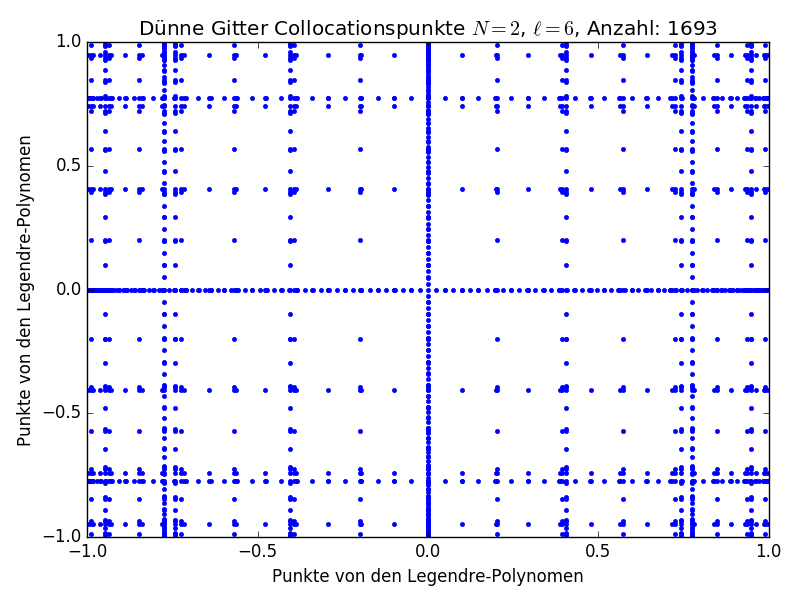
\includegraphics[width=\linewidth]{Figures/sparse_grid_legendre_legendre.png}
\endminipage
\minipage{0.5\textwidth}
  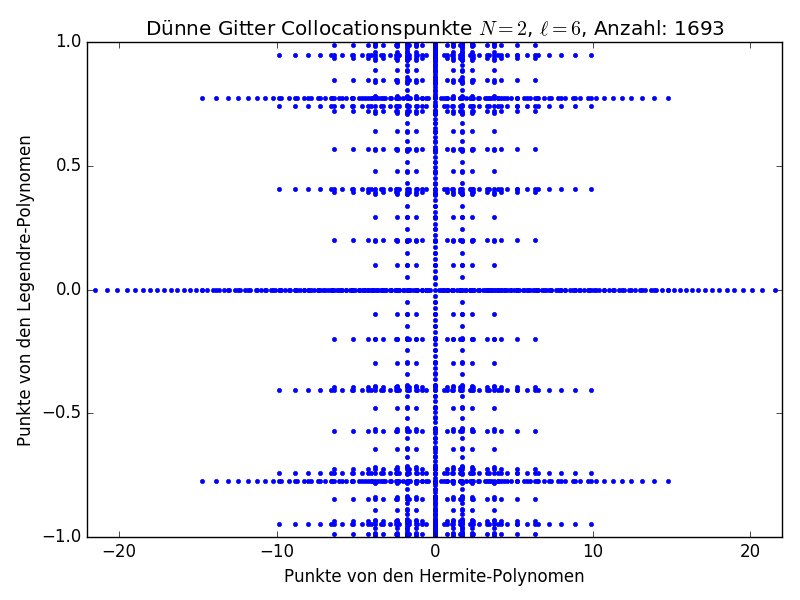
\includegraphics[width=\linewidth]{Figures/sparse_grid_hermite_legendre.png}
\endminipage
\caption{Dünne Gitter nach Smolyak mit $N=2$ und Legendre- bzw. Hermite-Collocationspunkten für das Level $\ell=6$.}
\label{fig:grids}
\end{figure}
Die Nullstellen der Legendre- und Hermite sind schwach geschachtelt (engl. \emph{weakly nested}), da für ungerade Polynomgrade die Zahl $0$ eine Nullstelle ist. Dies ist jedoch die einzige Wiederholung eines Knotenpunktes. Die Nullstellen der Laguerre- und Jacobi-Polynome besitzen im Allgemeinen keinerlei Schachtelung.\\
Im Gegensatz zu Gittern, die beispielsweise auf Glenshaw-Curtis Knotenpunkten basieren und vollständig geschachtelt sind, bieten schwach geschachtelte Gitter somit wenig Zeitersparnis durch Wiederverwendung von Collocationspunkten. Der Vorteil liegt hauptsächlich in der geschickten Approximation des vollen Tensorprodukts der exakten Operatoren.\\
Eine Implementierung für vollständig geschachtelte, schwach geschachtelte und nicht geschachtelte dünne Gitter in Matlab und C++ ist durch die Sandia Sparse Bibliothek (siehe \autocite{Sandia}) gegeben. Die Schwierigkeit liegt dabei darin, für schwach geschachtelte Gitter die einzelnen wieder auftauchenden Knotenstellen korrekt zu identifizieren.
\begin{figure}[!htb]
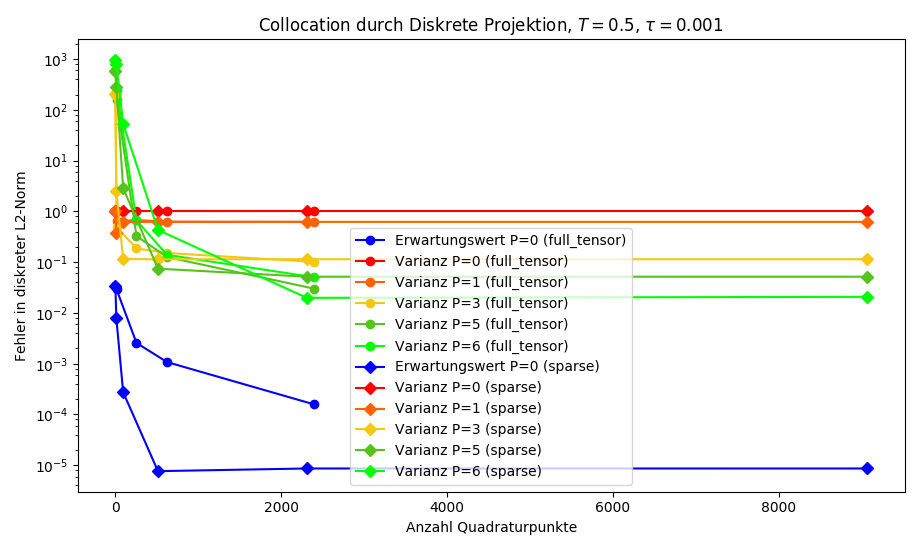
\includegraphics[width=\textwidth]{Figures/collocation_dp_trial8.png}
\caption{Konvergenz des Erwartungswert und der Varianz mit diskreter Projektion für \nameref{trial:8} mit $N=4$.}
\label{fig:dp_trial8}
\end{figure}
In Abbildung \ref{fig:dp_trial8} wird die Konvergenz der diskreten Projektion für das volle Tensorprodukt und den dünne Gitter Ansatz miteinander verglichen. Der Fehler wird dabei in Abhängigkeit von den Anzahl an benötigten Quadraturpunkten gezeigt. Wir beobachten:
\begin{itemize}
\item Der Erwartungswert benötigt nur $P=0$ und ist lediglich abhängig von der Güte der verwendeten Quadraturformel.
\item Der dünne Gitter Ansatz nach Smolyak ist für den Erwartungswert mit 1000 Quadraturpunkte in der Referenzgenauigkeit $\mathcal{O}(10^{-5})$ auskonvergiert.
\item Die maximal mögliche Genauigkeit der Varianz ist abhängig von $P$. 
\item Für größeres $P$ ist der Fehler der Varianz geringer, allerdings gilt dies erst, wenn die Quadraturformel die zusätzlich unter dem Integral auftauchenden Polynome $\Phi_m$ für $|m|=P$ exakt integriert.
\item Bei der Varianz zeigt der dünne Gitter Ansatz keine klaren Vorteile, da der Gesamtfehler stärker von $P$ als vom Quadraturfehler abhängig ist.
\item Will man die Varianz besser approximieren, so benötigt man mehr Koeffizienten $\hat{w}_m^{(j)}=\sum_{i=0}^Qu(t,x_j,y_i)\Phi_m(y_i)a_i$. Dies bedeutet, dass mehr Quadraturformeln durchgeführt werden müssen, die Collocationsstellen $u(t,x_j,y_i)$, die unabhängig von $m$ sind, allerdings wieder verwendet werden können.
\end{itemize} 

\subsubsection*{Glenshaw-Curtis Quadratur}
Die Glenshaw-Curtis Quadratur basierend auf den Knotenpunkten 
\[y_i=\cos\left(\frac{(n-1-i)\pi}{n-1}\right)\in[-1,1],\quad n\ge 2, i=0,\dots,n-1\]
ist eine häufig genutzte Quadraturformel mit vollständig geschachtelten Quadraturpunkten. Die Gewichte lassen sich in $\mathcal{O}(n\log n)$ Schritten berechnen.\\
Diese Quadratur ist für das kompakte Intervall $[-1,1]$ ausgelegt. Für die Legendre-Polynome und die Jacobi-Polynome mit $\alpha,\beta>0$ stimmt der Träger mit dem Träger der zugehörigen stochastischen Verteilung überein. Es gilt
\[\\E[Y]=\int_{[-1,1]}f(y)\rho(y)dy\approx\sum_{i=0}^Qf(y_i)\rho(y_i)a_i\]
Die Dichte $\rho$ wird hier explizit ausgewertet und ist nicht Teil der Quadraturformel, wie dies bei der Gauss-Quadratur der Fall war.\\
Für Hermite-Polynome mit zugehörigem Träger $(-\infty,\infty)$ bzw. Laguerre-Polynome mit zugehörigem Träger $(0,\infty)$ ist daher eine Transformation des Integrals nötig. Da $[-1,1]$ kompakt ist existiert aber keine Bijektion zwischen den Mengen. Heuristische Ansätze wie das Ignorieren der Randpunkte und anschließender Verwendung des Transformationssatzes auf $(-1,1)$ liefert schlechte Approximationen.\\
Unseren Beobachtungen nach bietet die Glenshaw-Curtis Quadratur keine Vorteile gegenüber der Gauss-Quadratur. Die polynomiale Exaktheit ist lediglich $n$ bei $n$ Quadraturpunkten und verwendet die Dichtefunktion der Verteilung nicht implizit. Die Dichte muss somit ebenfalls durch die Quadratur approximiert werden, was den nötigen Polynomgrad noch weiter erhöht. Schlussendlich erhöhen die Polynome $\Phi_m$, die bei der Approximation der Varianz unter dem Integral auftauchen, die benötigte polynomiale Exaktheit.
\subsection{Algorithmus}
Algorithmus \ref{alg:collocation_dp} skizziert die Berechnung der Approximation von Erwartungswert und Varianz mithilfe von Collocation durch diskrete Projektion.
\begin{algorithm}[ht]
    \caption{Collocation durch diskrete Projektion.}
    \label{alg:collocation_dp}
    \begin{algorithmic}[1] % The number tells where the line numbering should start
        \Function{Collocation\_Diskrete\_Projektion}{$H, u_0, v_0, \alpha,\beta,\kappa,Y, M, Q,\tau, T$} 
            \State $\Phi_m\gets$ $m$-te orthonormale gPC-Basis-Funktion zu $Y$, $\quad m=0,\dots,M$
            \State $a_i, y_i\gets$ (multivariate) Quadraturformel (siehe Kapitel \ref{chapter:multivariatequad}), $\quad i=0,\dots,Q$
            \For{$i=1,\dots,S$}
           		\State $\tilde{u}_{ij}\gets \text{Fast\_Strang}(H,u_0(\cdot, y_i),v_0(\cdot, y_i),\alpha(y_i),\beta(\cdot, y_i),\kappa,\tau,T)_j$
           	\EndFor
            \State $\hat{w}_m^{(j)}\gets \sum_{i=0,\dots,Q}\tilde{u}_{ij}\Phi_m(y_i)a_i$
			\State $\mu\gets \hat{w}_{0,j=1,\dots,H}$ \Comment{Approximation an Erwartungswert}
			\State $\sigma^2_j\gets \sum_{m=1,\dots,M}\hat{w}^2_{mj}$\Comment{Approximation an Varianz an der Stelle $x_j$}
			\State \textbf{return} $\mu,\sigma^2$ \Comment{Approximation an Erwartungswert und Varianz}        
        \EndFunction
    \end{algorithmic}
\end{algorithm}
\section{Vergleich der Ansätze Interpolation und diskrete Projektion}
In diesem Abschnitt werden wir die beiden Ansätze für die Collocation miteinander vergleichen. Dabei werden wir für die Interpolation die Gauss-Stützstellen verwenden und ebenso für die diskrete Projektion die Gauss-Quadratur. Wir betrachten Beispiele mit $N=1$ und $N=4$ und verwenden im mehrdimensionalen Fall den vollen Tensorprodukt Ansatz. Für die mehrdimensionale Quadratur bei der diskreten Projektion vergleichen wir zusätzlich den vollen Tensorprodukt Ansatz mit der dünnen Gitter Quadratur nach Smolyak.
\subsection*{Allgemeiner Vergleich}
\begin{center}
\begin{tabular}{p{0.47\linewidth}|p{0.47\linewidth}}
Interpolation & Diskrete Projektion\\
\hhline{=|=}
\multicolumn{2}{c}{Für Gauss-Stützstellen im Eindimensionalen äquivalent (siehe Satz \ref{th:interpol_and_proj})}\\
\hline
Collocationspunkte "'beliebig"' & Collocationspunkte entsprechen Quadraturpunkten\\
\hline
Benötigt Interpolationspunkte & Benötigt zusätzlich Quadraturgewichte zu Quadraturpunkten\\
\hline
Informationen über Stabilität durch Matrixkondition & Explizite Berechnung ohne gekoppeltes System\\
\hline
Erwartungswert abhängig von $P$ & Erwartungswert benötigt nur $P=0$\\
\hline
Bei quadratischer Matrix Varianz nur von $P$ abhängig & Varianz abhängig von $P$ und $Q$\\
\hline
Volles Tensorprodukt macht LGS überbestimmt & Volles Tensorprodukt ohne Stabilitätseinfluss\\
\end{tabular}
\end{center}
Die Überbestimmtheit des Systems bei der Interpolation mit vollem Tensorprodukt der Knoten ist bedingt durch unsere Wahl der Interpolationspolynome. Bei Verwendung des vollen Tensorprodukts der eindimensionalen Polynombasen ist diese Quelle der Instabilität auf Kosten der Rechenzeit beseitigt.\\
Dass für die Berechnung des Erwartungswerts nur $P=0$ benötigt wird, macht die diskrete Projektion für manche Anwendungen sehr attraktiv. Die explizite Berechnung der Koeffizienten, die ohne Lösen eines LGS auskommt, verspricht mehr Stabilität und Geschwindigkeit.\\
Die Beziehung der beiden freien Parameter $P$ für den eindimensionalen Polynomgrad und $Q$ für die Quadraturpunkte ist einerseits aus praktischer Sicht problematisch, da im Vorhinein unklar ist, welche Erhöhung eine Verbesserung der Approximation bietet. Andererseits ist der Einfluss der Parameter auf den Fehler durch die Aufteilung in den Fehler der Bestapproximation und den Aliasing Fehler aus theoretischer Sicht gut verstanden.
\subsection*{Numerischer Vergleich}

\subsubsection*{Eindimensionaler Fall anhand von \nameref{trial:7}}
Wir sehen in Abbildung \ref{fig:collocation_comparison_trial7} für den eindimensionalen Fall die Äquivalenz der diskreten Projektion und der Interpolation bei Verwendung von Nullstellen der orthogonalen Polynome als Collocationspunkte. Die Äquivalenz ist dann gegeben, wenn die Anzahl verwendeter Polynome $P+1$ der Anzahl verwendeter Quadraturpunkte $Q+1$ entspricht.
\begin{figure}[!htb]
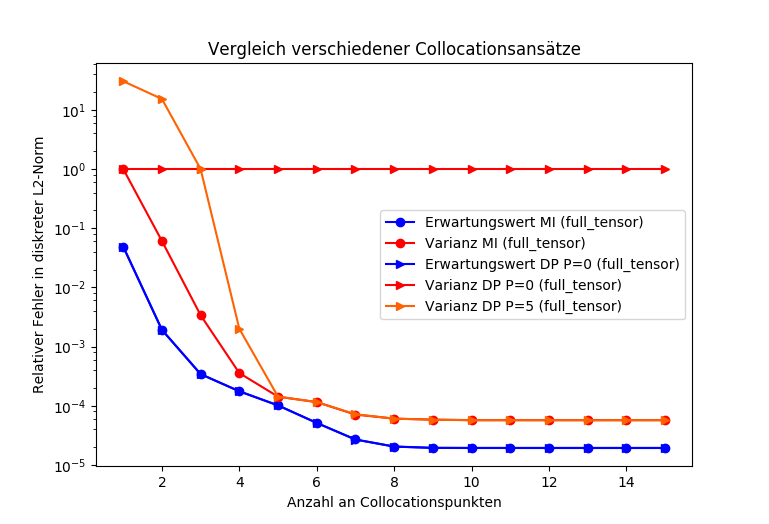
\includegraphics[width=\textwidth]{Figures/collocation_midp_trial7.png}
\caption{Konvergenz der Collocation für \nameref{trial:7} mit $N=1$ anhand der Anzahl benötigter Collocationspunkte.}
\label{fig:collocation_comparison_trial7}
\end{figure}

\subsubsection*{Vierdimensionaler Fall anhand von \nameref{trial:8}}
Wir sehen in Abbildung \ref{fig:collocation_comparison_trial8} den vierdimensionalen Fall. Hier ist der Erwartungswert wiederum für beide Ansätze gleich gut approximierbar unter Verwendung des vollen Tensorprodukts. Die dünne Gitter Quadratur bietet für den Erwartungswert klare Vorteile in Bezug auf die benötigten Collocationspunkte.\\
Bei der Interpolation lässt sich die Varianz wegen des überbestimmten Systems nicht zuverlässig berechnen. Bei der diskreten Projektion ist die Konvergenz in $P$ vergleichsweise langsam.
\begin{figure}[!htb]
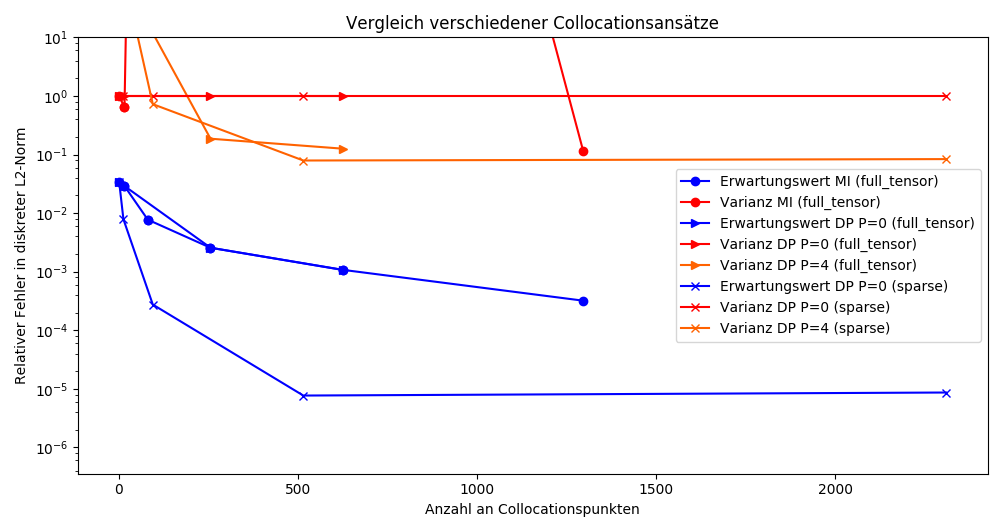
\includegraphics[width=\textwidth]{Figures/collocation_midp_trial8.png}
\caption{Konvergenz der Collocation für \nameref{trial:8} mit $N=4$ anhand der Anzahl benötigter Collocationspunkte.}
\label{fig:collocation_comparison_trial8}
\end{figure}

\subsubsection*{Unstetige Koeffizienten im Eindimensionalen}
Abbildung \ref{fig:collocation_comparison_trialdiscontsimple} zeigt für $N=1$ ein Beispiel, wo die Koeffizienten $\alpha$ und $\beta$ unstetig in $y$ sind. Dabei ist für $y\in[-1,1]$
\begin{align*}
\alpha(y)&=\begin{cases}2,\quad y>0\\ 1, \quad y\le 0\end{cases}\\
\beta(x,y)&=\begin{cases}2+\sin(x+y),\quad y>0\\ 2+\cos(x+y),\quad y\le 0\end{cases}\\
\end{align*}
Wir erkennen ein unterschiedliches Verhalten für eine gerade bzw. ungerade Anzahl an Quadraturpunkten, die im Eindimensionalen einer gerade bzw. ungerade Anzahl an Basispolynomen entsprechen. Für eine gerade Anzahl an Polynomen konvergieren Erwartungswert und Varianz vergleichbar mit bisherigen Beispielen.
\begin{figure}[!htb]
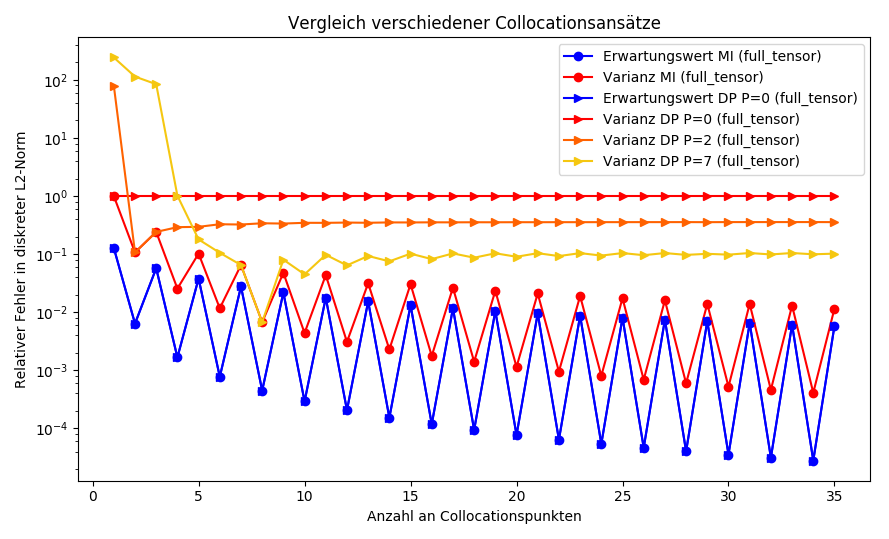
\includegraphics[width=\textwidth]{Figures/collocation_midp_trialdiscontsimple.png}
\caption{Konvergenz der Collocation für \nameref{trial:discontsimple} mit $N=1$ anhand der Anzahl benötigter Collocationspunkte.}
\label{fig:collocation_comparison_trialdiscontsimple}
\end{figure}
Fügen wir in \nameref{trial:disconttriple} eine weitere Unstetigkeitsstelle für $\alpha$ hinzu und entfernen die Unstetigkeit für $\beta$, so ist in Abbildung \ref{fig:collocation_comparison_trialdisconttriple} nur noch mit großer Mühe ein Konvergenzverhalten zu erkennen.
\begin{figure}[!htb]
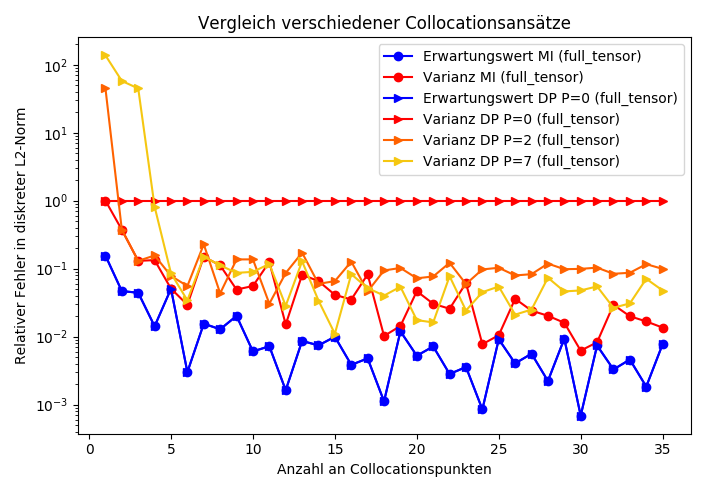
\includegraphics[width=\textwidth]{Figures/collocation_midp_trialdisconttriple.png}
\caption{Konvergenz der Collocation für \nameref{trial:disconttriple} mit $N=1$ anhand der Anzahl benötigter Collocationspunkte.}
\label{fig:collocation_comparison_trialdisconttriple}
\end{figure}
Für solche Probleme bieten sich adaptive Quadratur- und Interpolationsverfahren an, welche den Träger an bekannten oder unbekannten (Unstetigkeits)stellen aufteilen. Dafür ist es hilfreich die Theorie des gPC auf stückweise Polynome zu erweitern und entsprechende Quadraturverfahren zu verwenden.

